\documentclass[14pt, a4paper, oneside]{extarticle}
\usepackage[T2A]{fontenc}
\usepackage[utf8]{inputenc}
\usepackage[russian]{babel}
\usepackage{hyperref}
\usepackage{xcolor}
\usepackage{geometry}
\geometry{top=0.5cm, bottom=0.5cm, left=1cm, right=1cm}
\usepackage{graphicx}
\usepackage{float}
\usepackage{wrapfig}
\usepackage{fontawesome5}
\usepackage{ragged2e}
\usepackage{microtype}

\hypersetup{
    colorlinks=true,
    allcolors=blue,
    pdfborderstyle={/S/U/W 0},
    allbordercolors=blue
}

\begin{document}

% Фото

%\begin{wrapfigure}{l}{0.18\textwidth}
%	\vspace{\intextsep}
%    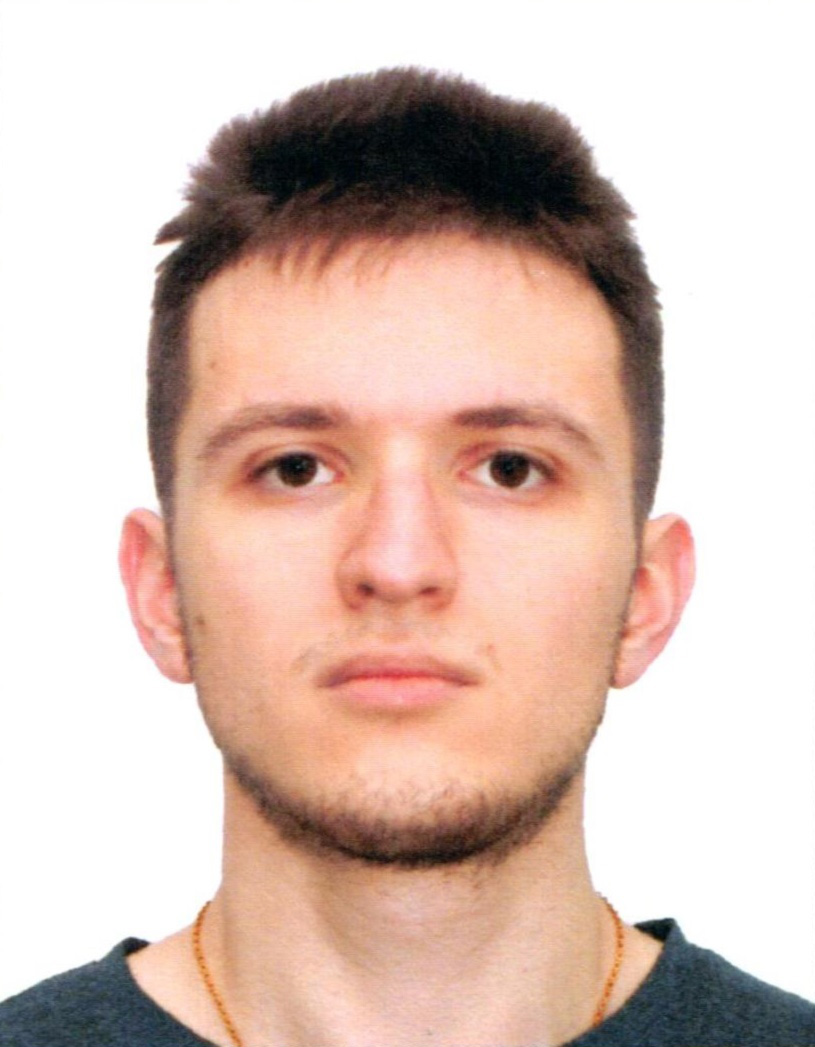
\includegraphics[width=0.18\textwidth]{personal_photo.jpg}
%\end{wrapfigure}

% Заголовок

\begin{center}
    \textbf{\LARGE Куценко Максим Дмитриевич}
    
    \textit{\Large Инженер данных}
\end{center}

\begin{center}
	\vspace{-0.5\intextsep}
	\small
    \faPhone* \space +7 (985) 647-53-50 | \faEnvelope \space maximkuts23@gmail.com | \faGithub \space github.com/Crazy5202 | \faTelegram \space @Crazy523
\end{center}

% Подзаголовок Практический опыт

\begin{flushleft}
	\vspace{-\intextsep}
	\large Практический опыт
\end{flushleft}

\vspace{-0.8\intextsep}
\hrule

%% eComm

\begin{flushleft}
	\vspace{-0.8\intextsep}
	\quad
	\href{https://github.com/Crazy5202/eComm}{\textbf{Бэкенд интернет-магазина (учебный проект)}}
	\hfill
	Москва
\end{flushleft}

\begin{flushleft}
	\vspace{-1\intextsep}
	\quad
	\textit{Московский авиационный институт}
	\hfill
	\textit{\small Фев. 2025 - Июнь 2025}
\end{flushleft}

%%% Список eComm

\begin{itemize}
	\vspace{-2\intextsep}
	\item \href{https://github.com/Crazy5202/job_application_form/tree/main/portfolio/eComm_C4.pdf}{Микросервисная архитектура}: 4 контейнера PostgreSQL с паттерном Database per service, контейнер Elasticsearch, контейнер S3, 4 контейнера инструментов наблюдаемости (Promtail, Prometheus, Loki, Grafana) 
	\vspace{-0.8\intextsep}
	\item Проектирование схем БД и миграций (PostgreSQL, SQLAlchemy, Alembic)
	\vspace{-0.8\intextsep}
	\item ETL/CDC пайплайн: синхронизация изменений в основной БД PostgreSQL с Elasticsearch через Debezium и Kafka для полнотекстового поиска продуктов
	\vspace{-0.8\intextsep}
	\item Визуальный анализ информации о метриках и логах через \href{https://github.com/Crazy5202/job_application_form/tree/main/portfolio/eComm_Grafana.pdf}{дашборд в Grafana}
\end{itemize}

%% Кинотеатр

\begin{flushleft}
	\vspace{-\intextsep}
	\quad
	\href{https://github.com/Crazy5202/Python_project}{\textbf{Онлайн-кинотеатр (учебный проект)}}
	\hfill
	Москва
\end{flushleft}

\begin{flushleft}
	\vspace{-1\intextsep}
	\quad
	\textit{Московский авиационный институт}
	\hfill
	\textit{\small Сент. 2024 - Дек. 2024}
\end{flushleft}

%%% Список Кинотеатр

\begin{itemize}
	\vspace{-2\intextsep}
	\item Batch ETL пайплайн: сбор HTML-страниц фильмов из IMDB по HTTP,
    парсинг информации, выгрузка в БД PostgreSQL и S3-хранилище
\end{itemize}

% Подзаголовок Конкурсы и достижения

\begin{flushleft}
	\vspace{-\intextsep}
	\large Конкурсы и достижения
\end{flushleft}

\vspace{-0.8\intextsep}
\hrule

%% K2

\begin{flushleft}
	\vspace{-0.8\intextsep}
	\quad
	\textbf{AI Boostcamp}
	\hfill
	Москва
\end{flushleft}

\begin{flushleft}
	\vspace{-1\intextsep}
	\quad
	\textit{К2 Нейротех}
	\hfill
	\textit{\small Нояб. 2025 - Дек. 2025}
\end{flushleft}

%%% Список K2

\begin{itemize}
	\vspace{-2\intextsep}
	\item Проектирование \href{https://github.com/Crazy5202/job_application_form/tree/main/portfolio/K2/RAG_C4.pdf}{архитектуры} и \href{https://github.com/Crazy5202/job_application_form/tree/main/portfolio/K2/RAG_DFD.pdf}{потока данных} эталонной RAG-системы
	\vspace{-0.8\intextsep}
    \item Создание функционирующей RAG-системы с n8n
\end{itemize}

% Подзаголовок Навыки

\begin{flushleft}
	\vspace{-\intextsep}
	\large Навыки
\end{flushleft}

\vspace{-0.8\intextsep}
\hrule

%% Навыки

\vspace{0.5\intextsep}

\textbf{БД и хранилища:} PostgreSQL, ClickHouse, S3, Elasticsearch, MongoDB, Redis

\textbf{Обработка данных и Big Data:} Apache Spark (PySpark, Spark SQL)

\textbf{Языки и инструменты:} SQL, Python (SQLAlchemy, Alembic, asyncio, pytest)

\textbf{Очереди и интеграции:} Kafka, RabbitMQ, Debezium, REST, JSON

\textbf{Инфраструктура:} Linux, Git, Docker, CI/CD

\textbf{Наблюдаемость:} Grafana, Prometheus, Loki

\textbf{Моделирование:} ERD, C4, DFD

\textbf{Трекинг и документация:} Jira, Confluence

\textbf{ИИ-инструменты:} n8n, ZCode 

\textbf{Методологии:} Scrum, Kanban

\textbf{Иностранные языки:} Английский C1

% Подзаголовок Образование

\begin{flushleft}
	\vspace{-\intextsep}
	\large Образование
\end{flushleft}

\vspace{-0.8\intextsep}
\hrule

%% Магистратура

\begin{flushleft}
	\vspace{-0.8\intextsep}
	\quad
	\textbf{Московский авиационный институт}
	\hfill
	Москва
\end{flushleft}

\begin{flushleft}
	\vspace{-\intextsep}
	\quad
	\textit{\footnotesize Магистр, фундаментальная информатика и информационные технологии} 
	%искусственный интеллект и суперкомпьютерное моделирование}
	\hfill
	\textit{\small Авг. 2026 - н.в.}
\end{flushleft}

%% Бакалавриат

\begin{flushleft}
	\vspace{-0.8\intextsep}
	\quad
	\textbf{Московский авиационный институт}
	\hfill
	Москва
\end{flushleft}

\begin{flushleft}
	\vspace{-\intextsep}
	\quad
	\textit{Бакалавр, прикладная математика и информатика}
	\hfill
	\textit{\small Авг. 2022 - Авг. 2026}
\end{flushleft}

% Подзаголовок О себе

\begin{flushleft}
	\vspace{-\intextsep}
	\large О себе
\end{flushleft}

\vspace{-0.8\intextsep}
\hrule

%% О себе
\begin{sloppypar}
	\vspace{0.5\intextsep}
	\quad
	Инженер данных с опытом проектирования БД и миграций в микросервисной среде, разработки ETL/CDC-пайплайнов и использования ИИ-инструментов. Обладаю опытом взаимодействия с командой разработки (от 4 до 9 человек), поддержки ТЗ.
\end{sloppypar}

\end{document}